\documentclass[conference]{IEEEtran}
\IEEEoverridecommandlockouts
\usepackage{cite}
\usepackage{amsmath,amssymb,amsfonts}
\usepackage{algorithmic}
\usepackage{graphicx}
\usepackage{textcomp}
\usepackage{caption}
\usepackage{hyperref}
\usepackage{booktabs}
\usepackage{amsmath}
\usepackage{subcaption}
\def\BibTeX{{\rm B\kern-.05em{\sc i\kern-.025em b}\kern-.08em
    T\kern-.1667em\lower.7ex\hbox{E}\kern-.125emX}}
\begin{document}

\title{Soil Classification Using Convolution
Neural Network}

\author{\IEEEauthorblockN{1\textsuperscript{st} Kaniz Reza Mithila}
\IEEEauthorblockA{\textit{Computer Science and Engineering (of Aff.)} \\
\textit{East West University (of Aff.)}\\
Dhaka, Bangladesh \\
2022-3-60-052@std.ewubd.edu}}

\maketitle


\textit{\textbf{Abstract—The research paper focuses on predicting soil types using Convolution Neural Network techniques and it help identifying different types of soil from images. In the paper, worked on 2 different soil image dataset. For analyzing soil, used four different models including two pre-trained model one is ResNet50 and another is VGG19 and also two custom-built CNN models. The dataset first dataset contains 1500+ images and the other one contains 4200+ images. After applying data augmentation, the dataset expanded images which helped improve model performance and generalization. During preprocessing image transforms and normalization were applied to both the validation and test sets to ensure consistent input quality. This made easier for the models to learn. The dataset was split into 70\% for training, 20\% for validation and 10\% for testing. The pre-trained models used transfer learning to reuse useful visual features learned from large datasets, while the custom models learned features directly from the soil images. ResNet50 performed the best, meaning it recognized soil types more accurately than the others. For better understanding used confusion matrices and curves to calculate the accuracy of the predictions that made by models.}}

\textit{\textbf{Keywords: Convolution Neural Network(CNN), Soil classification, Deep Learning, ResNet50, VGG19, Custom CNN model. }}

\section{Introduction}

Agriculture continues to play a fundamental role in the corroboration of food security and economic stability, especially in Bangladesh, where agriculture is a primary occupation. One of the key factors, which dominance agricultural productivity is soil quality. Each crop expands best under specific soil conditions. However, in our country many farmers still rely on traditional experience-based methods to identify soil types, which often leads to incorrect crop choices and reduced yield. With the assistance of digital technologies and convenient datasets, soil analysis has become a feasible way to shelter modern farming \cite{b1}. This problem becomes even bigger because different soils behave differently and farmers cannot identify their soil correctly, they often choose the wrong crop or use fertilizers in an unplanned way, leading to poor yields and long-term soil damage. Traditional soil testing needs lab facilities, takes time, and a huge part depends on manual judgment, which is not always accurate or affordable for everyone \cite{b8},\cite{b9}. With the assistance of digital technologies and convenient datasets, soil analysis has become a feasible way to shelter modern farming.

\begin{figure}[h]
    \centering
    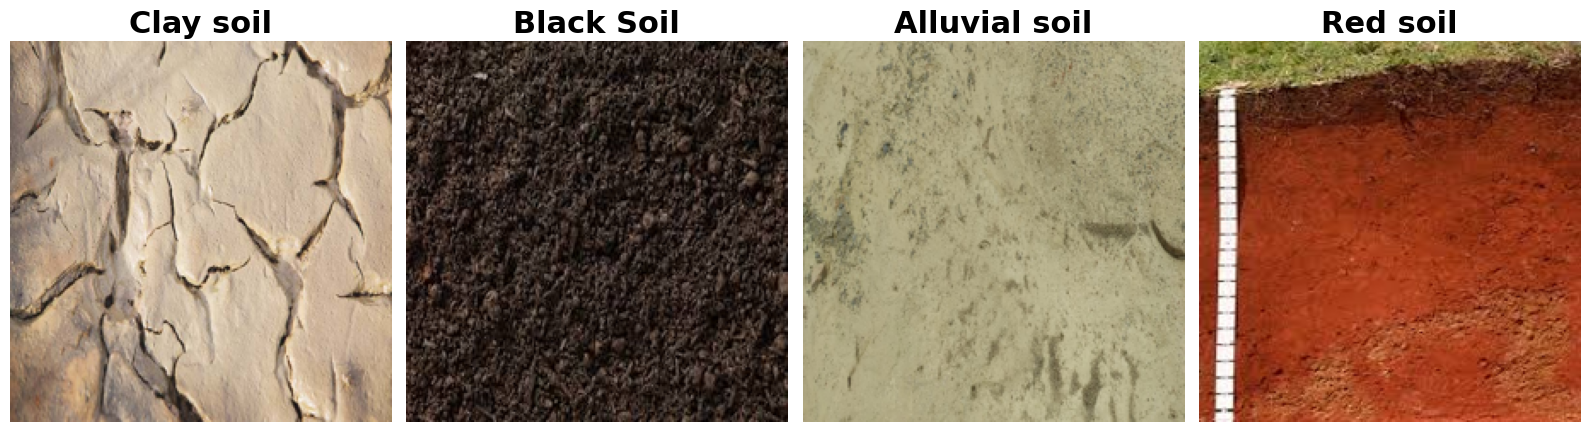
\includegraphics[width=0.48\textwidth]{figures/soil_image.png}
    \caption{Soil Images of Dataset 1}
    \label{fig:soil-images-d1}
\end{figure}

\begin{figure}[h]
    \centering
    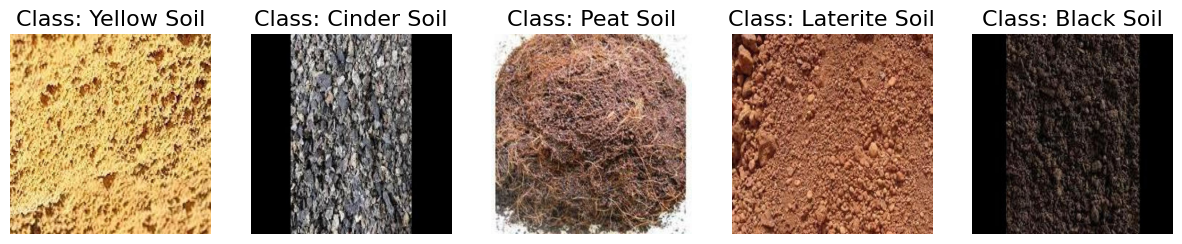
\includegraphics[width=0.48\textwidth]{figures/soil_image of dataset 2.png}
    \caption{Soil Images of Dataset 2}
    \label{fig:soil-images-d2}
    
\end{figure}
Recent deep learning have opened new possibilities for studying soil directly through images. Among these techniques, Convolutional Neural Networks (CNNs) have proven particularly effective at detecting the features in soil, such as texture, patterns, and colour variations, which are often difficult for humans to notice. Moat of the studies suggest that CNN-based models usually perform better than traditional machine learning approaches in soil and crop prediction tasks. This is mainly because CNNs learn directly from raw images instead of relying on handcrafted features, which can miss important details \cite{b6}.  The researchers shown that CNNs can achieve high accuracy when classifying different soil categories. It is performing better than previous methods such as SVM, Random Forest, and ANN models \cite{b2}. These results check CNNs as a strong and practical choice for building soil prediction tools. A study says multiple CNN architectures like custom CNN, ResNet50, InceptionV3, and MobileNetV2 were tested on a soil image dataset. The study found that ResNet50 have showed that the highest accuracy while the other models also performed very well. It shows that modern CNNs can capture different patterns effectively and can be reliable identify various soil types \cite{b7}. Overall, these findings reinforce the idea that CNNs are one of the most practical, accurate, and dependable options for real-world soil prediction systems.
\vspace{10pt}

This paper concentrates on developing a soil prediction model using two custom Convolutional Neural Networks (CNNs), ResNet50, VGG19 training on a soil image dataset. The intention is to create a system susceptible of identifying soil types from images and assisting farmers, students and researchers with reliable soil classification. By implementing deep learning into soil assessment, the objective of the proposed work is to contribute to precision agriculture and enhance more informed crop management decisions.


\section{Literature Review}
Soil classification has been explored through various machine learning and deep learning techniques in recent years. The researchers focused on using image-based methods to identify soil types more accurately than traditional approaches. The following review discusses key contributions and methods used in previous research.
\vspace{10pt}


The study introduces a deep learning based system. The research paper can identify soil types and suggest suitable crops using soil images. The researcher used a public Kaggle dataset containing more than 1,550 images of different soil types-alluvial, black, clay and red soils and implemented MobileNetV2 model. The result of MobileNetV2 model performed very well achieving 97.34\% accuracy training on dataset and 99.21\% accuracy validation dataset. In the end, the study concludes that this approach can be helpful for farmers choose the right crops for their soil. Which can lead to better crop yield and improved agricultural productivity.\cite{b1}.
\vspace{5pt}


This literature review begins with their study by reviewing earlier work. The paper explains how soil classification has shifted from manual to modern data driven approaches. Several studies experimented with models like SVM, Random Forest, KNN, and even smartphone-based colour sensors to make soil identification easier in the field. The paper supports their decision to compare ANN and CNN models for classifying four soil types from images. The CNN model performed better than the other proposed models, achieved 96\% acuuracy \cite{b2}.
\vspace{5pt}


After going through the paper, the authors relied on a Convolutional Neural Network (CNN) to classify different soil types.Their idea is to use soil images instead and let CNN pick up tiny visual details—like texture and color changes—that people might not notice easily.The authors mention that CNN gave the highest accuracy out of all the models they compared, which makes it a solid option for real farming work. Overall, the approach feels practical and more modern than the usual testing methods \cite{b3}.
\vspace{5pt}


A combination of XRF spectrum analysis and Random Forests, SVMs, and backpropagation neural networks (BPNN) brought about a discriminative rate of 99.62\%, 99.04\%, and 98.85\% respectively for soil classification \cite{b5}. Another approach, CNN utilizing the Inception V3 transfer learning model, had the remarkable result of 87.5\% accuracy in soil classification. Researchers using LUCAS soil dataset showed that CNNs could effectively bring about results of accuracy as high as 99.59\%. CNN models, such as VGG16, VGG19, Inception V3, and ResNet50 have been experimented with datasets and Inception V3 provided a satisfactory 87.53\% accuracy \cite{b4}.
\vspace{5pt}


Perez et al.\cite{b5} explore the problem of identifying soil ditches related to illegal underground tunnel activities based on remote sensing images. The difficulty is that the soil deposits outside got tunnel may look like same as natural topography and then it is difficult to detect by traditional image process methods. The authors employ a 4-layer CNN model trained with multispectral aerial images to classify the land patches into 14 categories, which includes disturbed soil. Their method includes methods for dealing with class imbalance, due to presence of few examples of excavated soil as opposed to background samples. With the paper mentioning that CNN properly extracts tunnel-affected areas, we cannot compare its performance to other models using numbers because there is no printed accuracy nor F1-score. Absence of transparency in dataset limit reproducibility \cite{b5}.
\vspace{5pt}


Sri et al. \cite{b6} deal with the problem of extracting soil type and crop prediction for automating farmers’ decision making through deep learning approaches. The authors suggest a CNN-adopted establishment to classify soil images at first and make suitable crop recommendations according to the prior knowledge of soil–crop following. This means no need for laborious soil testing and you're well on the way to your precision-farming regime. "Their approach focuses on combining soil type identification with practical crop-advisory systems. But there is a lack of open-access experimental details in the paper — no accuracy, dataset size, network depth and also confusion matrix are presented. In the absence of quantitative assessment, the true model performance cannot be verified or compared to similar CNN research. The lack of explanation also makes it harder to reproduce and benchmark datasets externally \cite{b6}.
\vspace{5pt}


The reviewing paper considers the problem of visual classification of soil types. This is An important task in planning for agriculture that is typically performed using expensive laboratory tests. They create image dataset consisting of more than 1800 soil images for popular categories of soils. The authors experiment with several deep-learning models, including a custom CNN, MobileNetV2, InceptionV3 and ResNet50. Of these, 97.3\% accuracy is achieved by ResNet50 implying the efficiency of transfer learning for soil-image classification. MobileNetV2 works well achieving 94.7\%, however it is a light-weight alternative that can be used in mobile applications. The major drawbacks are that the sample need to be large enough, which limits the use of spectral method under some circumstances, e.g., soil colour will change with moisture and lighting and impurity. However, the research contributes one of the best validated CNN benchmarks in soil classification work \cite{b7}.
\vspace{5pt}


Huang et al. \cite{b8} study the greater applicability of Convolutional Neural Networks for soil detection and explore how (also investigating the role of CNNs in identifying soil texture, contamination levels, moisture level and structure parameters. There is not a single experimental model, but several CNN models such as 5-layer CNNs and hybrids of CNN with optimization and pre-processing techniques are surveyed. Advances in stability, robustness and quality of feature extraction results are stressed by the authors to provide a deep learning update. But the paper does not provide a dataset or accuracy number in aggregated form, making it hard for others to compare with. The primary drawback of this method is that it rather serves as a review and concept demonstration than a quantitative assessment and does not provide quantifiable results and inherently cannot be easily compared across different researcher’s setups \cite{b8}.
\vspace{5pt}


In their article present an extensive review of the methods for soil identification and classification based on machine learning. They highlight the classical ML techniques, such as Support Vector Machines, Random Forest, and K-Nearest Neighbour, along with the coming deep learning techniques for soil property prediction. The review points out that soil classification has suffered from inconsistent datasets, environmental noise, and the absence of common benchmarks. Although the paper gives a review of the capabilities of the ML models, it does not put forward any new models or experimental configurations. Due to the fact that this work is based on a review, there are no accuracy statistics reported. The absence of summary tables or meta-analysis was a primary limitation that restricted the quantification of the contribution and knowing how much algorithmic performance (when applicable) has been added over previous work would have certainly strengthened the paper \cite{b9}.
\vspace{5pt}


Chatterjee et al. (2021)\cite{b10} addressed the issue of real-time soil type classification from pictures. They considered several different CNN architectures—ResNet50, VGG19, VGG16, MobileNetV2, NASNetMobile, and InceptionV3—on an enlarged image dataset comprising Clay, Black, Alluvial, and Red four soil types. As per the results they have reported, ResNet50 got the best training accuracy of around 99.47\% and was the one that defeated the others in terms of performance. The research provides evidence that the adoption of transfer-learning CNNs leads to reliable discrimination amongst soil types through image processing. However, one of the important drawbacks is that the only reported outcomes are training accuracy and loss—no public data is accessible regarding test accuracy, generalization for unseen data, or strong evaluation metrics are given. This paper clear doubts about the risk of overfitting and also whether the model would produce reliable results, in real-world soil images that come with unpredictable light, moisture or background conditions \cite{b10}.
\vspace{5pt}


This paper confronted the challenge of automatic soil image classification changing pictures of soils into soil-type labels so that they could replace the slow or lab-based methods of soil classification with automated ones. Their research combined different deep convolutional neural network (CNN) architectures to distinguish soils on the basis of image data. The later conversations summarizing their research found that a model like DenseNet201 was able to classify soil images with a very high accuracy of around 99.15\% on the soil-photo dataset. Although, such a remarkably high figure has prompted the question of overfitting if the dataset size, diversity, or external validation was limited which are the possible drawbacks for the application to real-world field scenarios. The positive side is the proof that deep CNNs can classify soil-images with outstanding accuracy under controlled conditions, the negative side is the uncertainty about generalizability without broader dataset evaluation or external validation \cite{b11}.
\vspace{5pt}


The paper work is all about the classification of soil types through machine learning techniques, which is an innovative approach that promises to be a scalable solution in the areas where traditional lab testing is not possible \cite{b12}. Their findings are also showing that their application focus is connected with the agriculture of developing regions. The authors opted for classical or machine-learning-based models and not deep CNNs, which is a symbol of the lightweight approach that is possible under limited computations. The downside is that there is no publicly available metadata for this paper that provides information on the dataset size, model architecture, accuracy, or confusion-matrix results. Consequently, the actual performance is still up for grabs. The situation is such that it becomes difficult to assess the quality of the method, or to compare it with other soil-classification studies; additionally, it hinders reproducibility and external validation. The study's merit is in the application of ML for soil classification in low-resource settings; however, it is limited by the lack of clarity regarding performance. The study's merit is in the application of ML for soil classification in low-resource settings; however, it is limited by the lack of clarity regarding performance \cite{b12}.
\vspace{5pt}


Zhan et al. (2023) target the practical problem of classifying excavated soils soil removed during construction or dredging and then transported which must be managed, reused, or disposed safely. Traditional lab-based soil classification is too slow or costly for large volumes; thus, they propose a multi-source data approach combining soil images, cone index (CI), dielectric constant (DC), and electrical conductivity (EC) measured via a Time-Domain Reflectometry (TDR) cone penetrometer, as features for classification. The core model is a CNN (specifically ResNet18) that processes image data along with the auxiliary sensor inputs \cite{b13}. On a large multi-source database (over 25,000 soil samples), their system classifies excavated soils into 12 types. The authors report an overall accuracy of 88.7\%, and for soils with “simple color patterns,” the accuracy reaches ~97\%. This demonstrates that combining visual and geotechnical data with deep learning can effectively classify excavated soils for reuse or disposal. The main limitation is reduced accuracy when soil color/patterns are complex which reflects challenges in real-world variability (moisture, mixtures, impurities) but the approach remains promising for large-scale soil management operations  \cite{b13}.
\vspace{5pt}


The research conducted by Hamzah et al. brings forward a novel idea of using deep learning to meet the challenges associated with classifying soil. As it has been identified that accuracy is a challenge for statistical and rule-based approaches, this research brings forward a Convolutional Neural Network (CNN) model to develop an accurate classification system. The researchers applied their deep learning approach and obtained a high accuracy rate of 97\% with a loss of 0.1606. Also, it performed well with an F1 score of 98\%. The study concludes that this deep learning approach effectively solves soil type classification issues, offering a more efficient alternative to conventional models \cite{b14}.
\vspace{5pt}


Building on the integration of classification and practical application, Girme et al. had developed an online system that, apart from classifying soils, recommends the corresponding crops. This online system uses a Convolutional Neural Network algorithm that classifies soils from their images. For instance, the CNN algorithm classifies Alluvial, Black, Clay, or Red soils. After the classification process, another algorithm called the Support Vector Machine recommends crops corresponding to the classified soil types. This system seeks to benefit farmers in their agricultural production decisions. Moreover, the system offers an online platform where farmers can market their produce \cite{b15}.
\vspace{5pt}


In the paper applies the concept of CNNs for the particular task of soil fertility evaluation through the analysis of remote sensing inputs. This particular task combines high-resolution Satellite imagery (Sentinel-2, ISRO BHUVAN), as well as drone images, for the evaluation and categorization of soil fertility levels into ‘high,’ ‘medium,’ and ‘low’ levels. To accomplish the task, the authors used the MobileNetV2 model as the foundation for extracting the features, gaining a validation accuracy of about 87 percent. This task automatically identifies patterns for soil texture and moisture without requiring manual feature identification for chemical analysis in laboratories, thus being an economical alternative for farmers and agricultural advisors for the chemical analysis of soil for agricultural farming inputs related to plant growth and development phases \cite{b16}.
\vspace{5pt}


The researcher address the problem of detecting soil productivity to distinguish between productive and unproductive land. Recognizing the limitations of manual laboratory classification, the authors created a substantial dataset comprising 31,600 training images and 6,320 testing images collected via mobile cameras across various districts in West Bengal. They tested CNN architectures such as AlexNet and VGG16 to predict soil fertility given image features such as color and texture. The CNN approach introduced better precision and recall over previous works, offering a sophisticated way to determine land quality \cite{b17}.
\vspace{5pt}


Moving on to the nutrient analysis component, Prajapati et al. performed a comparison between CNN and Linear Regression algorithms for the prediction of nutrient levels in the soil (N, P, K, and pH). Unlike conventional analysis that involves significant manual work, the current analysis involves an organized body of information regarding the characteristics of the soil. Notably, the comparison between the two algorithms revealed that CNN performed better compared to Linear Regression with an accuracy of 95.87\%, where the complex nutrient levels could not be effectively handled by Linear Regression analysis. This establishes the dominance of CNN even in non-image analysis nutrient levels assessment \cite{b18}.
\vspace{5pt}


Ballester et al. analyzed the aptness of Machine Learning algorithms to accurately determine the soil matric potential for a week. The experiment is based on data collected for six years on the cotton crop fields in Australia, taking into consideration the data collected on soils, weather, and satellite NDVI values. Of the several models analyzed, namely the LSTM model, Dense Multilayer Perceptron, Linear Regression, the model with the highest degree of predictability is the Convolutional Neural Network (CNN) model, with a difference in $R^2$ values of> = 0.92. The CNN model has the ability to identify a periodic trend, which can be correlated to irrigation and weather factors, making the model appropriate for irrigation-related decision-making \cite{b19}.
\vspace{5pt}


Correspondingly, a 1D CNN model for estimating SM was also proposed by Chen et al., using laboratory-scale Vis-NIR spectra. The 1D CNN model reported outstanding performance with an average $R^2$ value of 0.989. Notably, this research differed in incorporating a knowledge-based transfer learning approach, which helped to successfully adjust to novel target regions with varying soil background spectra. Notably, this approach of transfer learning increased the R2 value from 0.845 to 0.983 for unknown regions, performing better compared to basic PLS regression models \cite{b20}.
\vspace{5pt}


For remedying physical defects in soils, Andrushia et al. have proposed a deep learning-based solution to identify shrinkage cracks in expansive soils. The authors have established four models, namely two Customized CNN models, VGG-19, and ResNet-50. These have been established on an image dataset comprising 5,200 images collected from farmlands in India. It has been observed that their "Customized CNN Model 2" outperformed all other techniques or models in correctly identifying the crack patterns. This is representative of the fact that customized CNN architecture for certain geotechnical problems could be effective \cite{b21}.
\vspace{5pt}


Looking at earlier remote sensing methodologies, Dematte et al. focused on the detection and discrimination of bare soil in satellite images. Using the Landsat-5 TM image over the Brazilian region, they proposed a method based on discriminant analysis but not on deep learning techniques. They reported a correct assignment of 99.3 percent for soil categories. This foundational work gives a sense of how such early statistical spectral analysis has unfolded into the deep learning contemporary methods presented in the other references \cite{b22}.
\vspace{5pt}


Precision agriculture and the use of Deep Learning techniques have also been followed by researchers such as Fotabong et. al. who focused on the classification of soil automatically. The limitations posed by human labor-testing methodologies for soil classification, the researchers proposed and used the application of Convolutional Neural Networks. The dataset used involved soil images with 628 soil examples for training and test examples. The proposed CNN by the researchers performed extremely well, boasting an accuracy of 100\% for the validation set. The authors clearly clarified that their proposed CNN model has proven to offer considerably improved results compared to Artificial Neural Networks (ANN) and Linear SVM models \cite{b23}.
\vspace{5pt}


The work by Tziolas et al. brings into focus a new model development framework applied within Sentinel-2 multispectral data to predict the SOC content. The current researchers designed and proposed a multi-channel CNN that combined the reflection spectrum inputs with the spectrum converted by the pre-processing method. The spectral CNN provided an RMSE of 12.03 g C/kg, an $R^2$ of 0.64, and an RPIQ of 0.89. Later, aiming to boost the methodological accuracy, the authors also designed the DUPLICITE model, this is a dual input Deep Learning method that combined the spectral CNN features with the ANNs-preprocessed variables of environmental and topographic factors. The DUPLICITE model proved its superior predictive skills compared to the CNN, PLS, RF, SVM, and XGBOOST models, providing an RMSE of 11.60 g C/kg, an $R^2$ of 0.67, and an RPIQ of 0.92 \cite{b24}.
\vspace{5pt}


Matinfar et al. responded to the problem of identifying changes in soil salinization and mapping the cover in the arid regions of Ardakan, Iran. The authors employed Landsat MSS data from 1975 and Landsat TM data from 2004 for classifying different types of land cover, like salt crust, salty soils, as well as growth. They found that the overall classification accuracy for the Landsat TM image was 92\%, which rose above 90\% for every class when the results were combined with the addition of the thermal band. By comparing the maps derived from classifying the Landsat MSS data acquired in 1975 and Landsat TM data acquired in 2004, the authors were able to identify a variation in the cover of more than 39\%, which showed a considerable rise in salt crust expansion \cite{b25}.
\vspace{5pt}


Sridevy et al. discussed the application of various machine learning techniques to map soil properties. The paper analyzed a number of studies that employed models such as RF, SVM, ANN, and Cubist Regression. Reviewers have identified that the Machine Learning techniques generally outperform the conventional geostatistical methods by dealing with high-order and nonlinear datasets without strict statistical assumptions. For instance, Random Forest has often been reported as the most robust model for predicting soil nutrients such as nitrogen and carbon by yielding high $R^2$ values. One review indicated that deep learning methods like CNNs are emerging with regard to spectral analyses, which include Random Forest and Cubist, still have a wide applicability in digital soil mapping owing to handling various environmental covariates and resistance to overfitting \cite{b26}.
\vspace{0.3cm}


The reviewed studies showed that how deep learning, especially CNN-based models, can effectively identify and classify different soil types from images. Researchers suggest that larger datasets and advanced models can further enhance performance. This findings support the use of modern image techniques for soil analysis.
\vspace{5pt}                                  




\section{Proposed methodology}
In this study, two pre-trained CNN models were used-one is ResNet50 and another one is VGG19, alongside two custom CNN architectures to analyse soil images. All models were trained using the augmented dataset to ensure better generalization and reduce overfitting. Their performance was later evaluated using accuracy and loss curve, classification report and confusion matrix.

\begin{figure}[h]
    \centering
    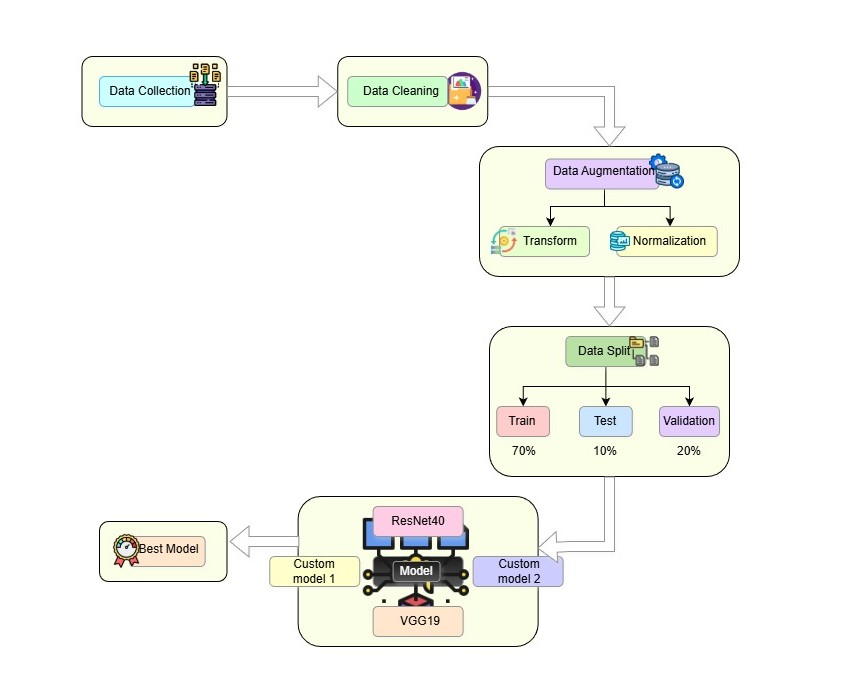
\includegraphics[width=0.4\textwidth]{figures/proposed image.jpeg}
    \caption{Overview of The Proposed Methodology}
    \label{fig:Overview of the proposed methodology}
\end{figure}

\subsection{Data collection and Processing}
For this study, soil image data was collected from Kaggle. The dataset is consisting of 1,550+ images representing four soil types-alluvial soil, black soil, clay soil and red soil.\cite{b2} For preparing the data for CNN model training, all the images were resized to 224×224 pixels to meet the input needs of the model \cite{b6}.The dataset was organized for training, validation and testing sets for ensuring  evaluation of model performance. This pre-processing ensure that all images were in same size and ready for accurately classification by the CNN models.

\subsection{Data Augmentation}
Data augmentation was used to the training dataset prevent overfitting and also improving the model generalization. The original dataset was limited so applied augmentation, helped to create additional and diverse samples without changing the class labels \cite{b6}.Augmentation used such as cropping and resizing, rotation, horizontal and vertical flips, affine transformations, perspective distortion, color jittering, Gaussian blurring, the custom unsharp mask, normalization and random erasing were used to simulate different image conditions and camera angles \cite{b7}. Finally, normalization was applied to standardize pixel values and stabilized training. These augmentation steps ensured the model learned features rather than memorizing the training images.

\begin{figure}[h]
    \centering
    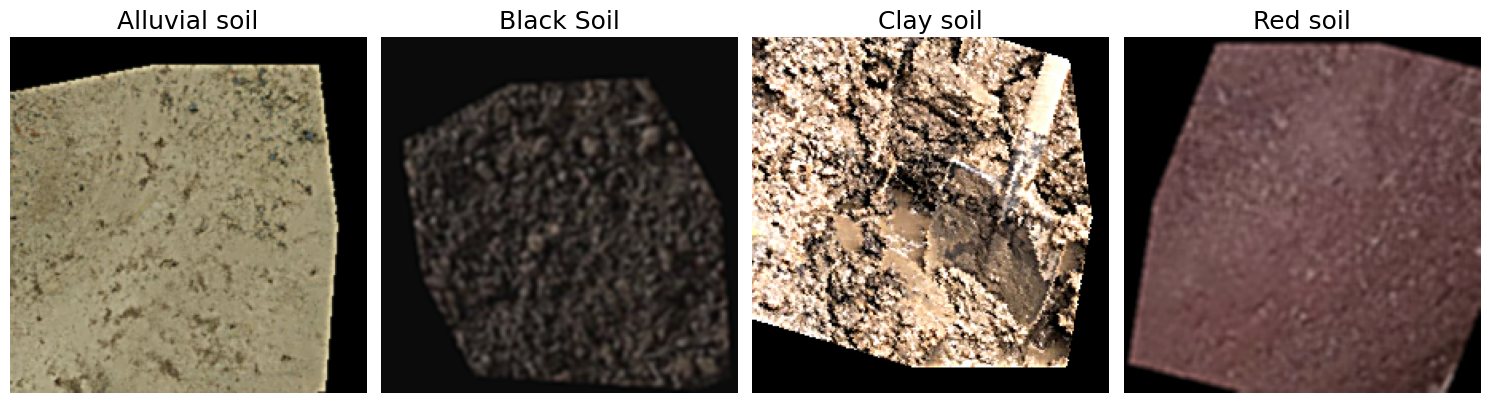
\includegraphics[width=0.48\textwidth]{figures/images after augmentation.png}
    \caption{Images After Augmentation of Dataset 1}
    \label{fig:images after augmentation of dataset 1}
\end{figure}

\begin{figure}[h]
    \centering
    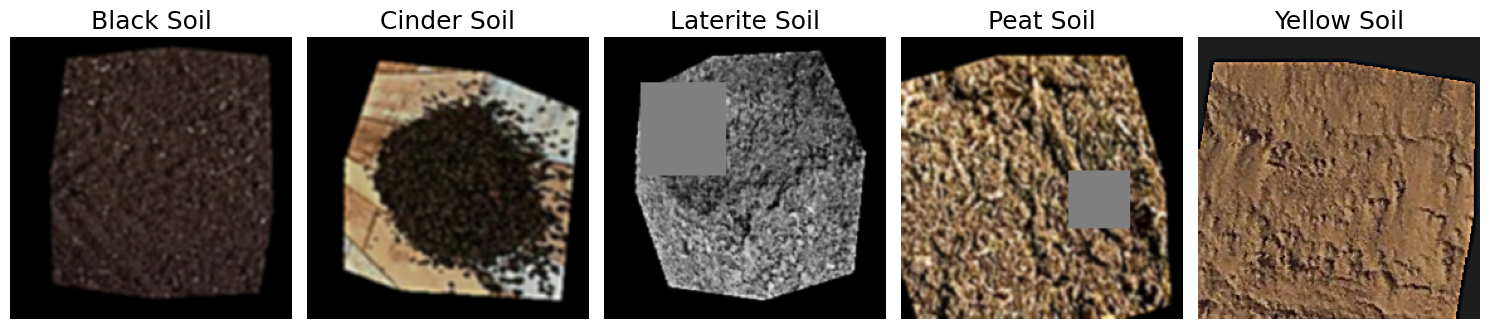
\includegraphics[width=0.48\textwidth]{figures/image after augmentation of dataset 2.png}
    \caption{Images After Augmentation of Dataset 2}
    \label{fig:images after augmentation of Dataset 2}
\end{figure}

\vspace{5pt} 
After augmentation dataset was imbalance, balanced classes only in training dataset. so that the model with a balanced balance training dataset exposure to all classes and improving its ability to generalize across both majority and minority classes.

\begin{figure}[h]
    \centering
    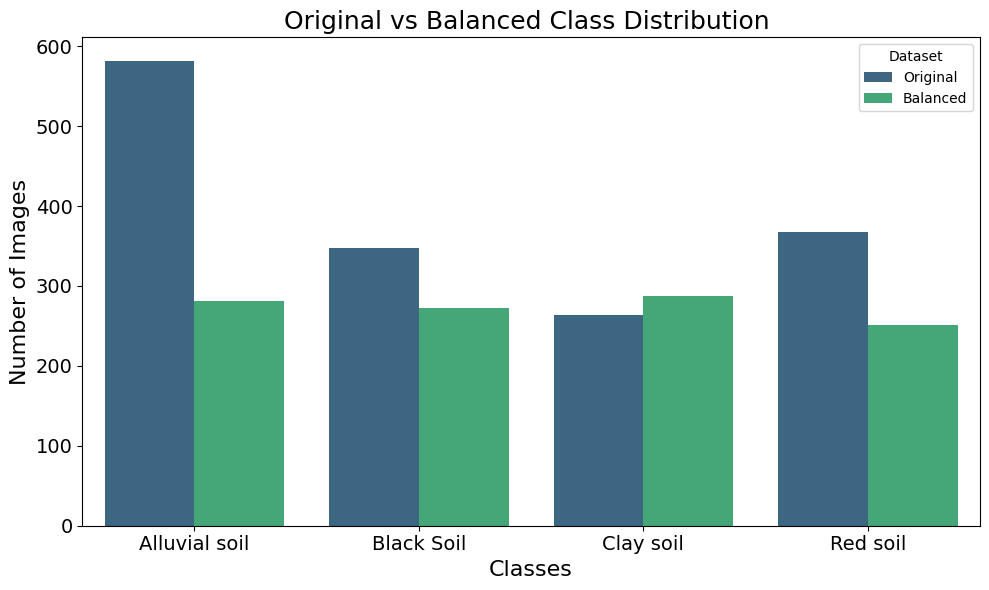
\includegraphics[width=0.48\textwidth]{figures/Original Dataset vs Balanced Class Distribution on Training Dataset.png}
    \caption{Original Dataset vs Balanced Class Distribution on Training Dataset of Dataset 1}
    \label{fig:Original Dataset vs Balanced Class Distribution on Training Datasetn}
\end{figure}


\begin{figure}[h]
    \centering
    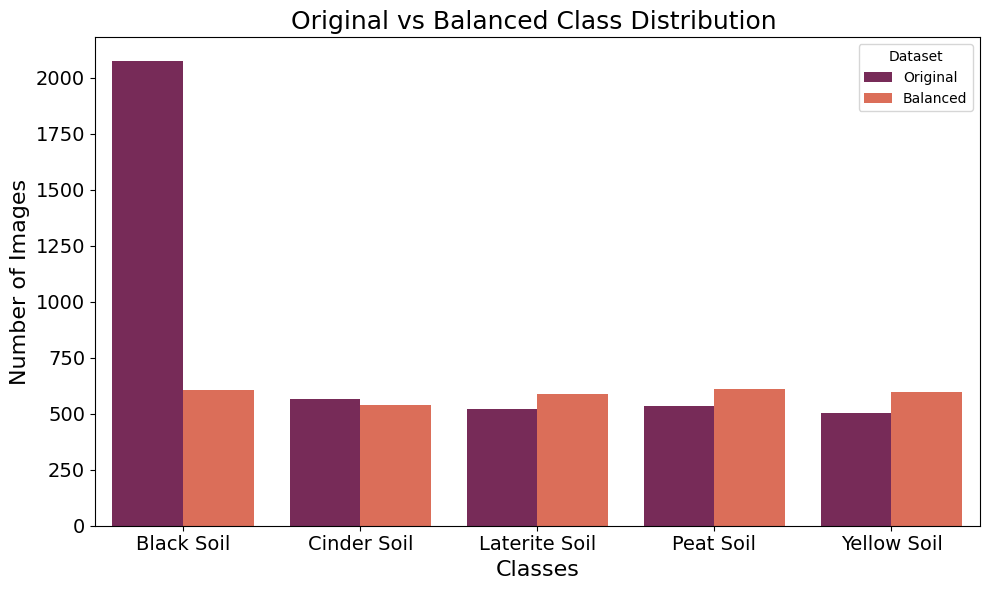
\includegraphics[width=0.48\textwidth]{figures/Original vs Balanced Class Distribution on Training Data of Dataset 2.png}
    \caption{Original Dataset vs Balanced Class Distribution on Training Dataset of Dataset 2}
    \label{fig:Original Dataset vs Balanced Class Distribution on Training Dataset of Dataset 2}
\end{figure}

\subsection{ResNet50}

In this study, the pre-trained model ResNet50 architecture was used for soil image classification for its strong ability to learn meaningful visual features from images. ResNet50 is built with residual blocks and skip connections that helps the model train deeper networks effectively without the problem of vanishing gradients. WeightedRandomSampler is used for balanceing classes on training dataset. This model was customized with 4 layers and the original fully connected layer was replaced with a new layer, which is containing four output neurons for representing the four soil classes-alluvial soil, black soil, clay soil, and red soil. The model was trained by using the Adam optimizer with a learning rate of 0.0001. The training process was used for batch size 32 and 20 epochs \cite{b10}. During the training, both training and validation accuracy were observed precisely for ensuring stable learning and consistent performance across different data splits. The images were provided to the model were resized to 224 × 224 pixels and that is the standard input size for ResNet50 models \cite{b10}\cite{b13}\cite{b7}. After completing the training process the model was tested on a separate test dataset to measure for real-world performance. The ResNet50 model achieved an outstanding 93.59\% test accuracy, showing excellent ability to correctly identify and differentiate between the four soil types. This high accuracy clearify the suitability of ResNet50 for soil classification tasks and the effectiveness of transfer learning in improving model performance.



\subsection{VGG19}
The model VGG19 is a deep convolutional neural network that contains 16 convolutional layers followed by 3 fully connected layers,  in total of 19 weight-bearing layers and one of the reasons it is widely used is because its structure is simple and consistent. Since it was trained on the large ImageNet dataset, This VGG19 model already knows how to detect general visual patterns like edges, curves, textures, and shapes. These basic features are also helpful for identifying differences among soil types \cite{b27}. In the work, loaded the pretrained version of VGG19 and froze the earlier convolutional layers. Freezing the early layers for helping the basic feature-extracting parts of the model for staying unchanged during training \cite{b12}. Also let the last layer unfreeze. It helps reduces training time and also helps prevent the model from overfitting. After that, replaced the final classifier with a new fully connected layer that outputs four classes which helps to match the soil categories in my dataset \cite{b10}. Also used the Adam optimizer with a learning rate of 0.0001 and the model was trained for 20 epochs. Also applied a learning-rate scheduler so that the learning rate slowly decreased.The VGG19 model achieved an outstanding 87.18\% test accuracy, showing excellent ability to correctly identify and differentiate between the four soil types. In the end, the VGG19 model performed well and showed that it can effectively learn the visual characteristics from different soil types of soil images.

\subsection{Custom Model 1}
In the work created a custom Convolutional Neural Network to classify the four soil types. The model is built with four convolutional layers that helps it learn different patterns from the images \cite{b6}\cite{b8}. And used epoch 20 and batch size 32. In the first layer picks up basic shapes and edges then the second layer learns stronger textures, third layer High-level feature extraction and the forth layer identifies more detailed soil features. Every layer of MaxPooling step reduces image size that makes the model faster which helps to prevent overfitting. LeakyReLU are used to help the model learn non-linear patterns more accrately.
Once the model finishes extracting features it starts flattens the output and passes it through two fully connected layers. In first dense layer has 128 units and Dropout of 0.3 which randomly turns off some neurons, during training to improve generalization. The final layer predicts which soil category the image is in which class \cite{b3}. This model was trained by using PyTorch. And adjusted to the number of soil classes in the dataset. This custom CNN provides a simple and effective approach for soil classification using image features.

\subsection{Custom Model 2}
The second custom model is designed to learn soil features deeply and more detailed way than the first model. It is built with five convolutional layer and every layer contains two convolution layers that used by Batch Normalization \cite{b7}. Different activation functions are used across blocks, including LeakyReLU, ELU, and ReLU, to help the model learn patterns effectively. This helps the model learn patterns more smoothly and prevents issues. Each layer also MaxPooling that reduces image size and Dropout layers with increasing values oderly 0.2, 0.3, 0.4, 0.5 for reducing overfitting. In the final layer turns the feature into a shape which makes the model more efficient and stable during training \cite{b9}. After extracting features model moves into the classifier section and there the output is flattened and passed through two fully connected layers \cite{b4}. The first fully connected layer reduces the features to 256 units and uses LeakyReLU and Dropout 0.4. The final layer predicts the soil type based on the features. The model uses Adam optimizer with learning rate of 0.001 and scheduler to reduce the learning rate while training the data. This custom CNN is designed more deeper and more accurate for soil image classification.



\section{Result And Analysis}
To predicting soil type, used two pre-trained model and two custom model. The pre-trained model is RestNet50 and VGG19.
\vspace{5pt}

\begin{table}[h!]
\centering
\begin{tabular}{{|p{3cm}|p{2cm}|}}
\hline
\textbf{Model Name} & \textbf{Accuracy} \\ \hline
RestNet50 & 98.08\% \\ \hline
VGG19 & 94.87\% \\ \hline
Custom Model 1 & 88.46\% \\ \hline
Custom Model 2 & 83.97\%\\ \hline
\end{tabular}
\caption{Models With Test Accuracy of Dataset 1}
\label{tab:accuracy-d1}
\end{table}

\begin{table}[h!]
\centering
\begin{tabular}{{|p{3cm}|p{2cm}|}}
\hline
\textbf{Model Name} & \textbf{Accuracy} \\ \hline
RestNet50 & 98.81\% \\ \hline
VGG19 & 97.86\% \\ \hline
Custom Model 1 & 76.72\% \\ \hline
Custom Model 2 & 71.73\%\\ \hline
\end{tabular}
\caption{Models With Test Accuracy of Dataset 2}
\label{tab:accuracy-d2}
\end{table}

To predict soil types from images of two dataset, two models were pre-trained (ResNet50 and VGG19) and two were custom-built CNN models and Their test accuracies are shown in Table 1 and table 2.

\vspace{10pt}

For both of dataset, the ResNet50 model gave the highest accuracy, VGG19 also performed strongly and produced accuracy. This shows that pre-trained models are very good at recognizing image features because they have learned from large datasets. The custom models also performed well, but their accuracy was slightly lower. Custom Model 1 and Custom Model 2 also achieved good results, which indicates that its structure capable of capture soil details as clearly.
\vspace{5pt}


\begin{figure}[htbp]
     \centering
     % Left Subfigure
     \begin{subfigure}[b]{0.4\textwidth}
         \centering
         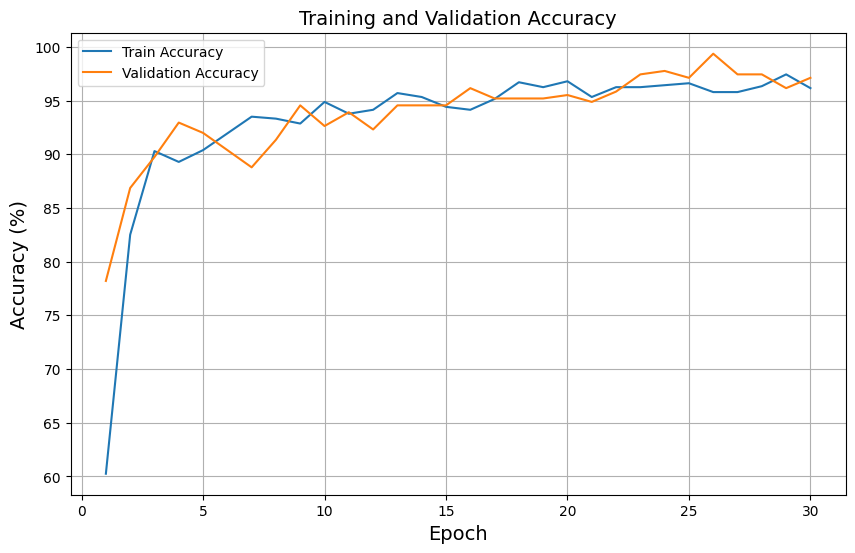
\includegraphics[width=\textwidth]{figures/Training and Validation Accuracy of RestNet50 Dataset 1.png}
         \label{fig:accuracy-resnet-d1}
     \end{subfigure}
     \hfill % Adds horizontal space between the two images
     % Right Subfigure
     \begin{subfigure}[b]{0.4\textwidth}
         \centering
         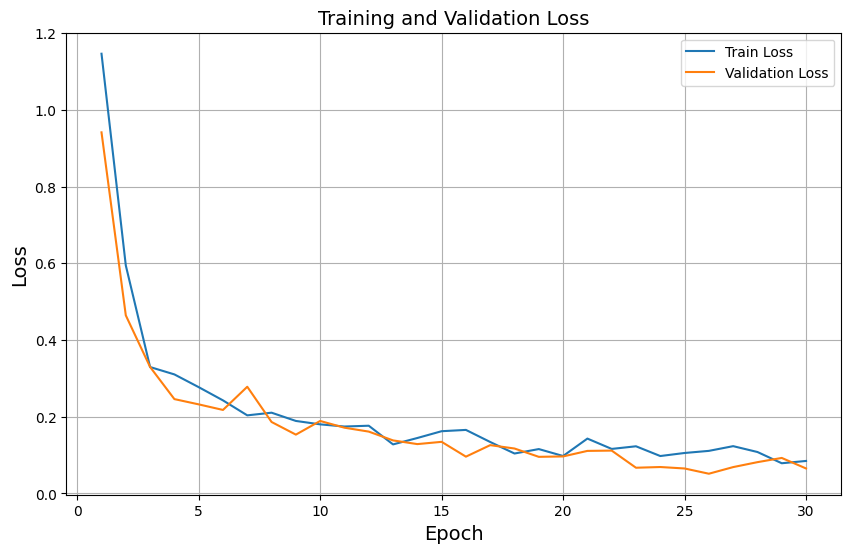
\includegraphics[width=\textwidth]{figures/Training and Validation Loss of RestNet50 dataset 1.png}
         \label{fig:loss-resnet-d1}
     \end{subfigure}
     
     \caption{Training vs Validation Accuracy and Loss curve of ResNet50 of Dataset 1.}
     \label{fig:Training vs Validation Accuracy and Loss curve of ResNet50 of Dataset 1}
\end{figure}



\begin{figure}[htbp]
     \centering
     % Left Subfigure
     \begin{subfigure}[b]{0.4\textwidth}
         \centering
         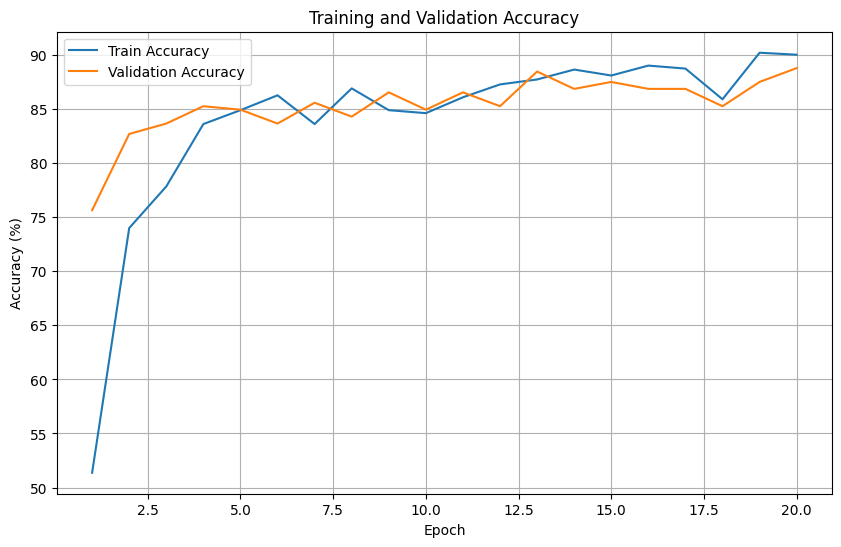
\includegraphics[width=\textwidth]{figures/Training and Validation Accuracy of VGG19.png}
         \label{fig:accuracy-vgg-d1}
     \end{subfigure}
     \hfill % Adds horizontal space between the two images
     % Right Subfigure
     \begin{subfigure}[b]{0.4\textwidth}
         \centering
         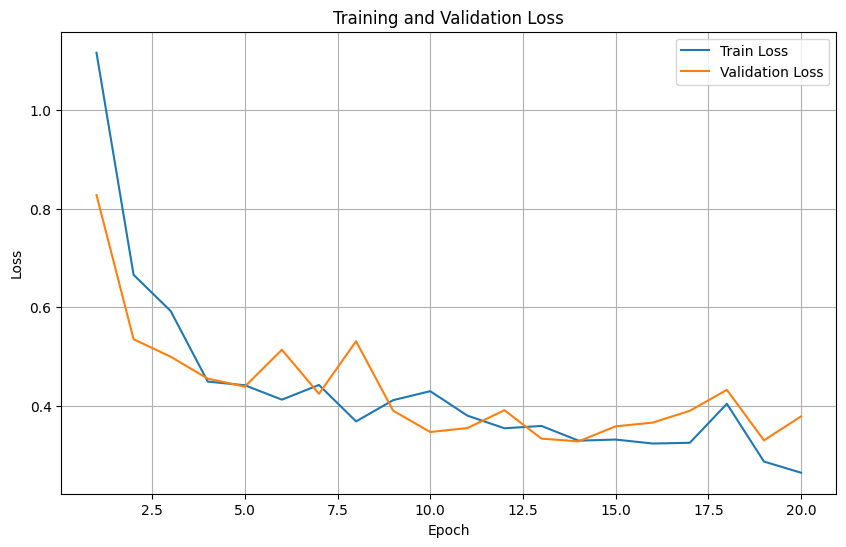
\includegraphics[width=\textwidth]{figures/Training and Validation Loss of VGG19.png}
         \label{fig:loss-vgg-d1}
     \end{subfigure}
     
     \caption{Training vs Validation Accuracy and Loss curve of VGG19 of Dataset 1.}
     \label{fig:Training vs Validation Accuracy and Loss curve of VGG19 of Dataset 1}
\end{figure}




\begin{figure}[htbp]
     \centering
     % Left Subfigure
     \begin{subfigure}[b]{0.4\textwidth}
         \centering
         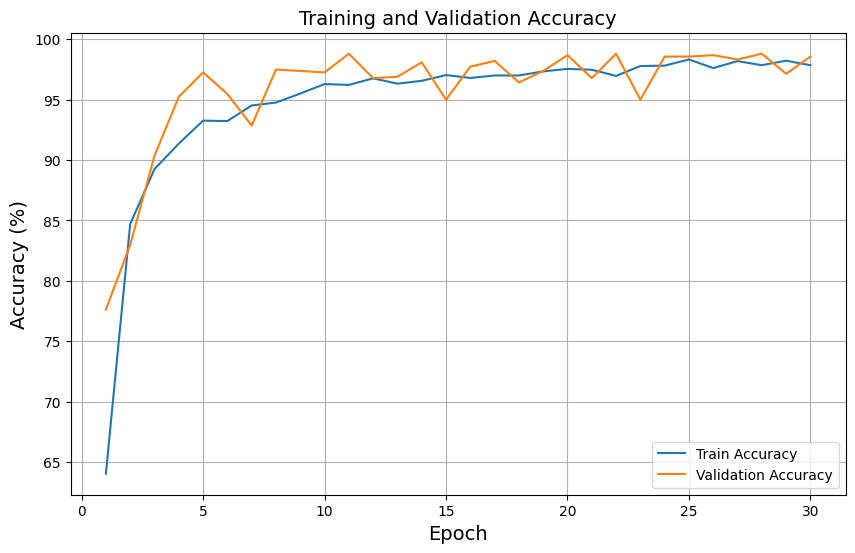
\includegraphics[width=\textwidth]{figures/Training and Validation Accuracy Curve of Resnet50 dataset 2.png}
         \label{fig:accuracy-resnet-d2}
     \end{subfigure}
     \hfill % Adds horizontal space between the two images
     % Right Subfigure
     \begin{subfigure}[b]{0.4\textwidth}
         \centering
         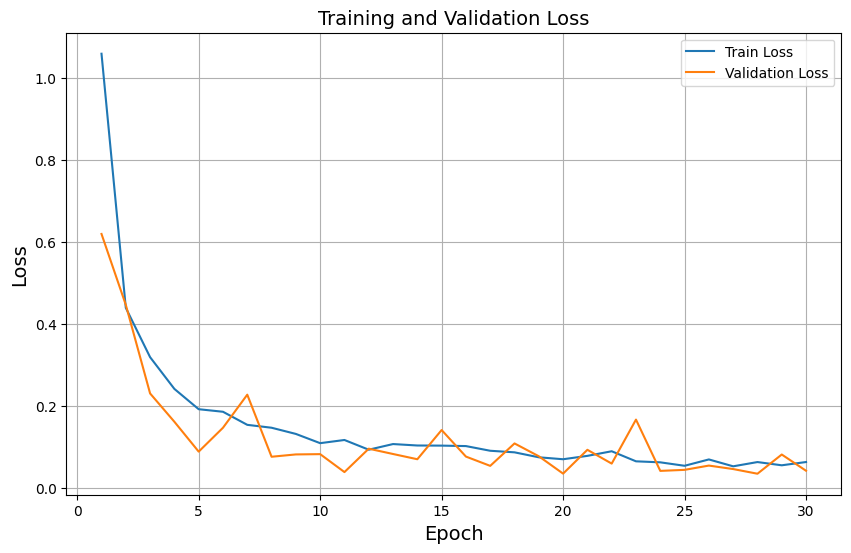
\includegraphics[width=\textwidth]{figures/Training and Validation Loss Curve of ResNet50 dataset 2.png}
         \label{fig:loss-resnet-d2}
     \end{subfigure}
     
     \caption{Training vs Validation Accuracy and Loss curve of ResNet50 of Dataset 2.}
     \label{fig:Training vs Validation Accuracy and Loss curve of ResNet50 of Dataset 2}
\end{figure}



\begin{figure}[htbp]
     \centering
     % Left Subfigure
     \begin{subfigure}[b]{0.4\textwidth}
         \centering
         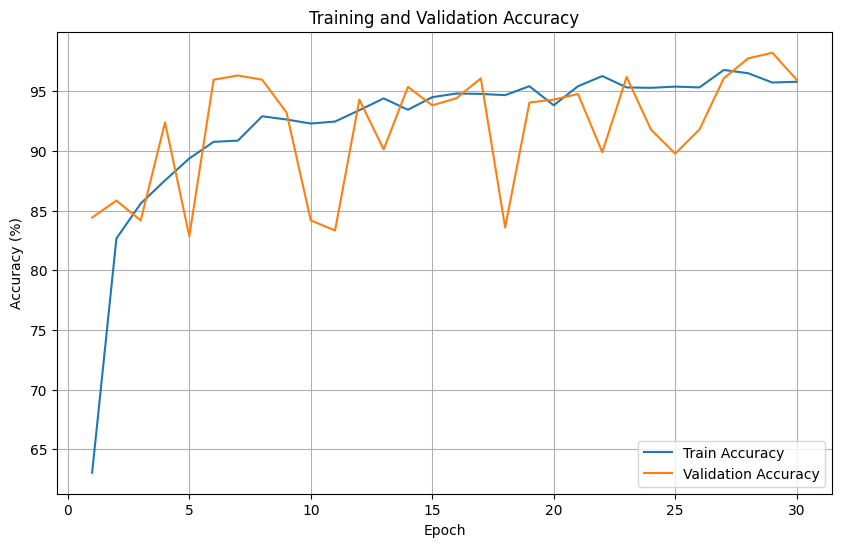
\includegraphics[width=\textwidth]{figures/Training and Validation Accuracy Curve of VGG19 of Dataset 2.png}
         \label{fig:accuracy-vgg-d2}
     \end{subfigure}
     \hfill % Adds horizontal space between the two images
     % Right Subfigure
     \begin{subfigure}[b]{0.4\textwidth}
         \centering
         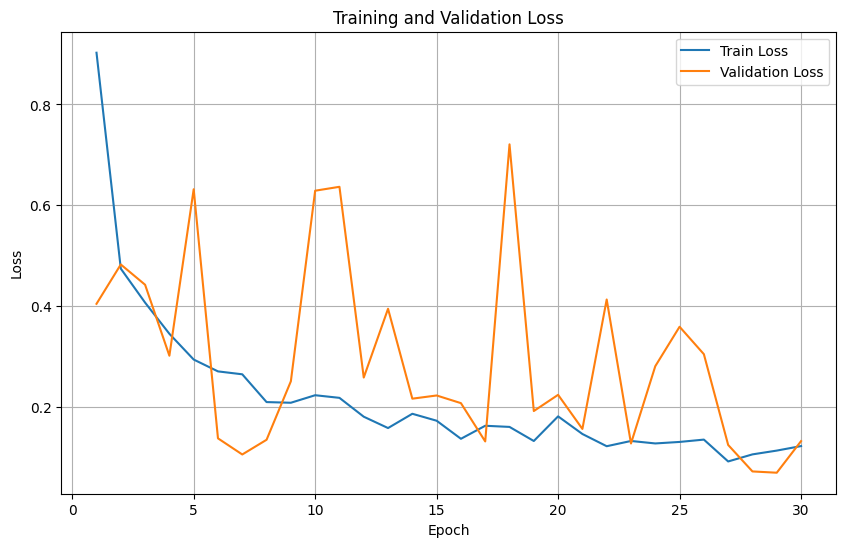
\includegraphics[width=\textwidth]{figures/Training and Validation Loss Curve of VGG19 of dataset 2.png}
         \label{fig:loss-vgg-d2}
     \end{subfigure}
     
     \caption{Training vs Validation Accuracy and Loss curve of VGG19 of Dataset 2.}
     \label{fig:Training vs Validation Accuracy and Loss curve of VGG19 of Dataset 2}
\end{figure}



\begin{table}[htbp]
    \centering

    % Subtable: Custom Model 1 
    \begin{subtable}{\columnwidth}
        \centering
        \begin{tabular}{lccc}
            \toprule
            \textbf{Class} & \textbf{Precision} & \textbf{Recall} & \textbf{F1-score} \\
            \midrule
            Alluvial soil & 0.8868 & 0.8545 & 0.8704 \\
            Black soil    & 1.0000 & 0.9167 & 0.9565 \\
            Clay soil     & 0.6786 & 0.7308 & 0.7037 \\
            Red soil      & 0.9286 & 1.0000 & 0.9630 \\
            \midrule
            \textbf{Accuracy} & & & \textbf{0.8846} \\
            Macro Avg     & 0.8735 & 0.8755 & 0.8734 \\
            Weighted Avg  & 0.8887 & 0.8846 & 0.8856 \\
            \bottomrule
        \end{tabular}
        \caption{Classification Report of Custom Model 1}
    \end{subtable}

    \vspace{5pt}

    % Subtable: Custom Model 2
    \begin{subtable}{\columnwidth}
        \centering
        \begin{tabular}{lccc}
            \toprule
            \textbf{Class} & \textbf{Precision} & \textbf{Recall} & \textbf{F1-score} \\
            \midrule
            Alluvial soil & 0.9286 & 0.7091 & 0.8041 \\
            Black soil    & 1.0000 & 0.9444 & 0.9714 \\
            Clay soil     & 0.6129 & 0.7308 & 0.6667 \\
            Red soil      & 0.7959 & 1.0000 & 0.8864 \\
            \midrule
            \textbf{Accuracy} & & & \textbf{0.8397} \\
            Macro Avg     & 0.8343 & 0.8461 & 0.8321 \\
            Weighted Avg  & 0.8593 & 0.8397 & 0.8404 \\
            \bottomrule
        \end{tabular}
        \caption{Classification Report of Custom Model 2}
    \end{subtable}

    \caption{Classification performance of Custom Models 1 and 2 of Dataset 1}
    \label{tab:overall_performance}
\end{table}



\begin{figure}[htbp]
     \centering
     % Left Subfigure
     \begin{subfigure}[b]{0.4\textwidth}
         \centering
         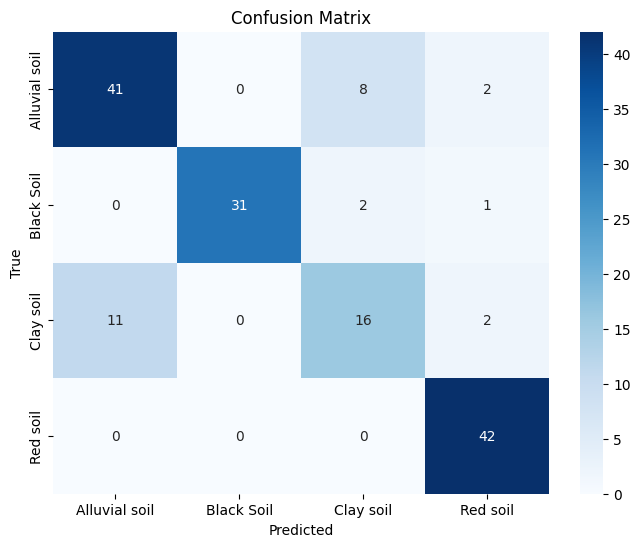
\includegraphics[width=\textwidth]{figures/Confusion Matrix of Custom Model 1.png}
         \label{fig:cm-custom1-d1}
     \end{subfigure}
     \hfill % Adds horizontal space between the two images
     % Right Subfigure
     \begin{subfigure}[b]{0.4\textwidth}
         \centering
         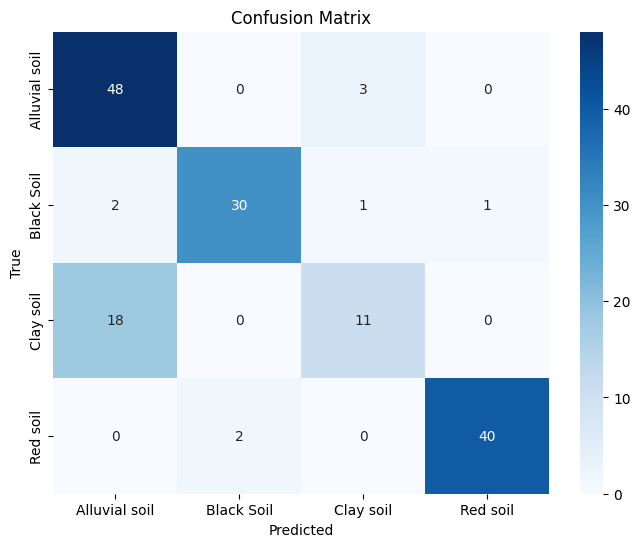
\includegraphics[width=\textwidth]{figures/Confusion Matrix of Custom Model 2.png}
         \label{fig:cm-custom2-d1}
     \end{subfigure}
     
     \caption{Confusion Matrix of Custom Model 1 and 2 of Dataset 1.}
     \label{fig:Confusion Matrix of Custom Model 1 and 2 of Dataset 1}
\end{figure}



\begin{table}[htbp]
    \centering

    % Subtable: Classification Report 1
    \begin{subtable}{\columnwidth}
        \centering
        \begin{tabular}{lccc}
            \toprule
            \textbf{Class} & \textbf{Precision} & \textbf{Recall} & \textbf{F1-score} \\
            \midrule
            Black Soil     & 0.9693 & 0.7560 & 0.8495 \\
            Cinder Soil    & 0.6944 & 0.5208 & 0.5952 \\
            Laterite Soil  & 0.8644 & 0.8947 & 0.8793 \\
            Peat Soil      & 0.4091 & 0.7143 & 0.5202 \\
            Yellow Soil    & 0.8302 & 1.0000 & 0.9072 \\
            \midrule
            \textbf{Accuracy} & & & \textbf{0.7672} \\
            Macro Avg      & 0.7535 & 0.7772 & 0.7503 \\
            Weighted Avg   & 0.8254 & 0.7672 & 0.7813 \\
            \bottomrule
        \end{tabular}
        \caption{Classification Report of Custom Model 1}
        \label{tab:model3}
    \end{subtable}

    \vspace{5pt}

    % Subtable: Classification Report 2
    \begin{subtable}{\columnwidth}
        \centering
        \begin{tabular}{lccc}
            \toprule
            \textbf{Class} & \textbf{Precision} & \textbf{Recall} & \textbf{F1-score} \\
            \midrule
            Black Soil     & 0.9627 & 0.7416 & 0.8378 \\
            Cinder Soil    & 0.8824 & 0.3125 & 0.4615 \\
            Laterite Soil  & 0.7869 & 0.8421 & 0.8136 \\
            Peat Soil      & 0.3571 & 0.6349 & 0.4571 \\
            Yellow Soil    & 0.6286 & 1.0000 & 0.7719 \\
            \midrule
            \textbf{Accuracy} & & & \textbf{0.7173} \\
            Macro Avg      & 0.7235 & 0.7062 & 0.6684 \\
            Weighted Avg   & 0.8042 & 0.7173 & 0.7278 \\
            \bottomrule
        \end{tabular}
        \caption{Classification Report of Custom Model 2}
        \label{tab:model4}
    \end{subtable}

    \caption{Classification performance of Custom Models 1 and 2 of Dataset 2}
    \label{tab:additional_models}
\end{table}


\begin{figure}[htbp]
     \centering
     % Left Subfigure
     \begin{subfigure}[b]{0.4\textwidth}
         \centering
         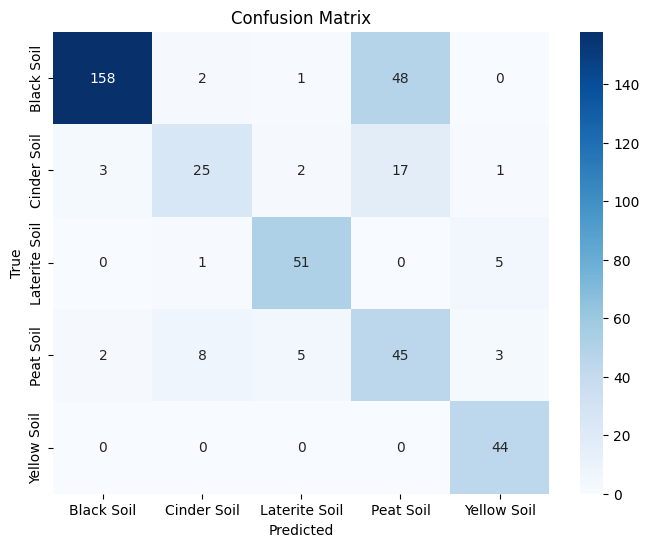
\includegraphics[width=\textwidth]{figures/Confusion Matrix of Custom Model 1 Of dataset 2.png}
         \label{fig:cm-custom1-d2}
     \end{subfigure}
     \hfill % Adds horizontal space between the two images
     % Right Subfigure
     \begin{subfigure}[b]{0.4\textwidth}
         \centering
         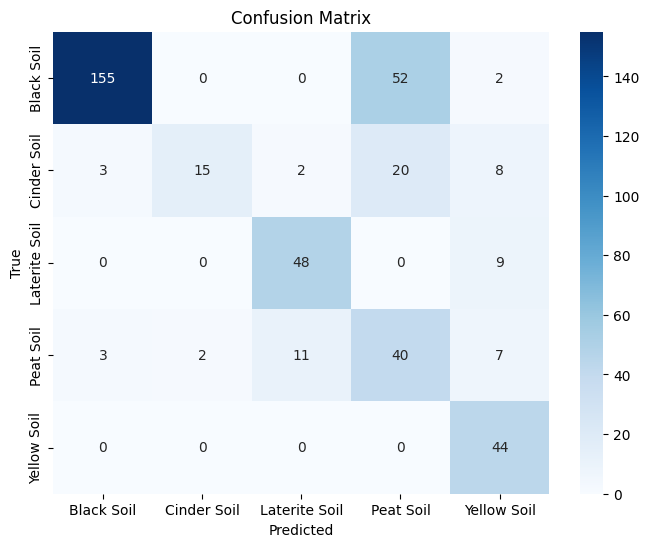
\includegraphics[width=\textwidth]{figures/Confusion Matrix of Custom Model 2 Of dataset 2.png}
         \label{fig:cm-custom2-d2}
     \end{subfigure}
     
     \caption{Confusion Matrix of Custom Model 1 and 2 of Dataset 2.}
     \label{fig:Confusion Matrix of Custom Model 1 and 2 of Dataset 2}
\end{figure}


Accuracy:
It defined as the number of correct predictions made as a ratio of all predictions made.
\begin{equation}
\text{Accuracy} = \frac{TP + TN}{TP + FP + FN + TN}
\end{equation}
\vspace{5pt}

precision:
The precision determines the proportion of positive prediction that was actually correct. It can be calculated as the True Positive or predictions that are actually true to the total positive predictions.
\begin{equation}
\text{Precision} = \frac{TP}{TP + FP}
\end{equation}
\vspace{5pt}

Recall:
It aims to calculate the proportion of actual positive that was identified incorrectly. It can be calculated as True Positive or predictions that are actually true to the total number of positives, either correctly predicted as positive
or incorrectly predicted as negative.
\begin{equation}
\text{Recall} = \frac{TP}{TP + FN}
\end{equation}
\vspace{5pt}

F-Score:
the F-score is a measure of a test's accuracy. It is calculated from the precision and recall of the test accuracy.
\begin{equation}
F1 - \text{score} = 2 * \frac{\text{precision} \cdot \text{recall}}{\text{precision} + \text{recall}}
\end{equation}
\vspace{10pt}

The classification report shows that the proposed custom models achieves good precision, recall, and F1-score across all classes, indicating reliable and balanced classification performance.


\section{conclusion}
Convolutional Neural Network model is represented in this paper which was specifically created to classify types of soil.This paper explores how well Convolutional Neural Networks (CNNs) can classify different soil types using images. In this study, worked with two pre-trained models one is ResNet50 another one is VGG19 and also worked with two CNN models that built from scratch. The pre-trained models used transfer learning. Which means they were already trained on large image datasets. so they could quickly pick up important features from the soil images. On the other hand, the custom models learned everything directly from the given dataset.Overall, the results show that CNN models can clearly detect small differences in soil texture, colour and patterns. This kind of automatic soil classification can help a lot in agriculture, land use planning and environmental work because it is faster. It can be used on a large scale, and gives more consistent results than checking soils by hand.

\section{Future Scope}
In the future, the models can be enhanced by integrating IoT sensors together for real-time soil information that will be improve prediction accuracy. Using more advanced deep learning models also can be explored to capture more precisely soil features. Additionally, already developing a mobile application will allow farmers to easily upload soil images and receive instant predictions. Working on more larger dataset and incorporating explainable AI techniques will be further strengthen the reliability and usability of the model.


\bibliographystyle{IEEEtran}
\bibliography{references}

\end{document}
